% questions.tex —— 2020 年·上海春季招生数学试卷 · 题目内容片段（无答案）
% 由 tools/generate_projects.py 依来源总账自 2020/2020_数学真题_春季上海_试题.md 生成，勿手改（改源 MD 后重跑）


\begin{gktip}
\textbf{来源边界}：题签见固定来源 PDF 第 1 页。固定 PDF 共 9 页：第 1–2 页为题面，第 3–9 页附有自称“参考答案与试题解析”的材料。上海市教育考试院同期点评中的题目特征与扫描件相合，可支持考试身份识别，但不证明该扫描件为官方发布原件，也不证明其发行版次、出版社或复制来源链。源附答案另行摘录与核对；本稿不将其标作官方答案。

\textbf{固定来源}：source ID \texttt{src-aacbb6140d9e12bc5aca908afe4d613b6ae584f08da89de4fa537d174727f9c2}；SHA-256 \texttt{4cb2e71aa66630c0154487dbb06436236701c22f79f770193436e20b60e9e327}。

\textbf{题面复核状态}：主会话依 PDF 页图逐题转录；第二位复核者只使用 PDF 第 1–2 页，逐题核对了题干、公式、选项、小问顺序及页码映射，未发现差异。独立解答不代表答案官方性核验。源页未明示的条件不擅自补入。
\end{gktip}

\gkpart{一、填空题}

\begin{gktip}
本大题共 12 题，满分 54 分；第 1–6 题每题 4 分，第 7–12 题每题 5 分。
\end{gktip}

\begin{question}
\gkti{1}集合 $A=\{1,3\}$，$B=\{1,2,a\}$，若 $A\subseteq B$，则 $a=\underline{\qquad\qquad}$。（PDF 第 1 页）

\end{question}
\begin{question}
\gkti{2}不等式 $\dfrac1x>3$ 的解集为 $\underline{\qquad\qquad}$。（PDF 第 1 页）

\end{question}
\begin{question}
\gkti{3}函数 $y=\tan 2x$ 的最小正周期为 $\underline{\qquad\qquad}$。（PDF 第 1 页）

\end{question}
\begin{question}
\gkti{4}已知复数 $z$ 满足 $z+2\overline z=6+i$，则 $z$ 的实部为 $\underline{\qquad\qquad}$。（PDF 第 1 页）

\end{question}
\begin{question}
\gkti{5}已知 $3\sin 2x=2\sin x$，$x\in(0,\pi)$，则 $x=\underline{\qquad\qquad}$。（PDF 第 1 页）

\end{question}
\begin{question}
\gkti{6}若函数 $y=a\cdot 3^x+\dfrac1{3^x}$ 为偶函数，则 $a=\underline{\qquad\qquad}$。（PDF 第 1 页）

\end{question}
\begin{question}
\gkti{7}已知直线 $l_1\colon x+ay=1$，$l_2\colon ax+y=1$，若 $l_1\parallel l_2$，则 $l_1$ 与 $l_2$ 的距离为 $\underline{\qquad\qquad}$。（PDF 第 1 页）

\end{question}
\begin{question}
\gkti{8}已知二项式 $(2x+\sqrt{x})^5$，则展开式中 $x^3$ 的系数为 $\underline{\qquad\qquad}$。（PDF 第 1 页）

\end{question}
\begin{question}
\gkti{9}三角形 $ABC$ 中，$D$ 是 $BC$ 中点，$AB=2$，$BC=3$，$AC=4$，则 $\overrightarrow{AD}\cdot\overrightarrow{AB}=\underline{\qquad\qquad}$。（PDF 第 1 页）

\end{question}
\begin{question}
\gkti{10}已知 $A=\{-3,-2,-1,0,1,2,3\}$，$a,b\in A$，则 $|a|<|b|$ 的情况有 $\underline{\qquad\qquad}$ 种。（PDF 第 1 页）

\end{question}
\begin{question}
\gkti{11}已知 $A_1,A_2,A_3,A_4,A_5$ 五个点，满足
\nopagebreak[4]
\[
\overrightarrow{A_nA_{n+1}}\cdot\overrightarrow{A_{n+1}A_{n+2}}=0\quad(n=1,2,3),\qquad
\left|\overrightarrow{A_nA_{n+1}}\right|\left|\overrightarrow{A_{n+1}A_{n+2}}\right|=n+1\quad(n=1,2,3),
\]
则 $\left|\overrightarrow{A_1A_5}\right|$ 的最小值为 $\underline{\qquad\qquad}$。（PDF 第 1 页）

\end{question}
\begin{question}
\gkti{12}已知 $f(x)=\sqrt{x-1}$，其反函数为 $f^{-1}(x)$，若 $f^{-1}(x)-a=f(x+a)$ 有实数根，则 $a$ 的取值范围为 $\underline{\qquad\qquad}$。（PDF 第 1 页）

\end{question}
\gkpart{二、选择题}

\begin{gktip}
本大题共 4 题，每题 5 分，共 20 分。
\end{gktip}

\begin{question}
\gkti{13}计算：$\displaystyle\lim_{n\to\infty}\frac{3^n+5^n}{3^{n-1}+5^{n-1}}=\left(\quad\right)$。（PDF 第 1 页）

\begin{gkopts}(4)
\task A．$3$
\task B．$\dfrac53$
\task C．$\dfrac35$
\task D．$5$
\end{gkopts}

\end{question}
\begin{question}
\gkti{14}“$\alpha=\beta$”是“$\sin^2\alpha+\cos^2\beta=1$”的\mbox{（　　）}。（PDF 第 1 页）

\begin{gkopts}(2)
\task A．充分非必要条件
\task B．必要非充分条件
\task C．充要条件
\task D．既非充分又非必要条件
\end{gkopts}

\end{question}
\begin{question}
\gkti{15}已知椭圆 $\dfrac{x^2}{2}+y^2=1$，作垂直于 $x$ 轴的垂线交椭圆于 $A$、$B$ 两点，作垂直于 $y$ 轴的垂线交椭圆于 $C$、$D$ 两点，且 $AB=CD$，两垂线相交于点 $P$，则点 $P$ 的轨迹是\mbox{（　　）}。（PDF 第 1 页）

\begin{gkopts}(4)
\task A．椭圆
\task B．双曲线
\task C．圆
\task D．抛物线
\end{gkopts}

\end{question}
\begin{question}
\gkti{16}数列 $\{a_n\}$ 各项均为实数，对任意 $n\in\mathbb N^*$ 满足 $a_{n+3}=a_n$，且行列式
\nopagebreak[4]
\[
\begin{vmatrix}a_n&a_{n+1}\\a_{n+2}&a_{n+3}\end{vmatrix}=c
\]
为定值，则下列选项中不可能的是\mbox{（　　）}。（PDF 第 1 页）

\begin{gkopts}(4)
\task A．$a_1=1,\ c=1$
\task B．$a_1=2,\ c=2$
\task C．$a_1=-1,\ c=4$
\task D．$a_1=2,\ c=0$
\end{gkopts}

\end{question}
\gkpart{三、解答题}

\begin{gktip}
本大题共 5 题，共 $14+14+14+16+18=76$ 分。
\end{gktip}

\Needspace{0.4\textheight}
\begin{question}
\gkti{17}\textbf{（14 分）} 已知四棱锥 $P-ABCD$，底面 $ABCD$ 为正方形，边长为 $3$，$PD\perp$ 平面 $ABCD$。（PDF 第 1 页）

（1） 若 $PC=5$，求四棱锥 $P-ABCD$ 的体积；

（2） 若直线 $AD$ 与 $BP$ 的夹角为 $60^\circ$，求 $PD$ 的长。
\nopagebreak[4]
\begin{center}% 2020 上海春季卷第 17 题；仅重绘原图可见线型与顶点标记，坐标为示意投影。
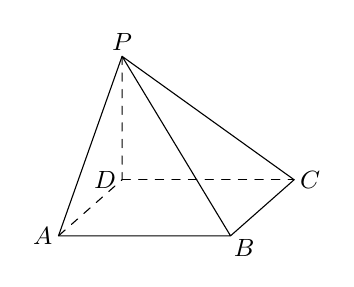
\begin{tikzpicture}[scale=.95,line cap=round,line join=round,font=\small]
  \coordinate (A) at (0,0);
  \coordinate (B) at (2.3,0);
  \coordinate (C) at (3.15,.75);
  \coordinate (D) at (.85,.75);
  \coordinate (P) at (.85,2.4);

  \draw[dashed] (P) -- (D) -- (A);
  \draw[dashed] (D) -- (C);
  \draw (P) -- (A) -- (B) -- (C) -- (P) -- (B);

  \node[above,inner sep=2pt] at (P) {$P$};
  \node[left,inner sep=2pt] at (A) {$A$};
  \node[below right,inner sep=1pt] at (B) {$B$};
  \node[right,inner sep=2pt] at (C) {$C$};
  \node[left,inner sep=2pt] at (D) {$D$};
\end{tikzpicture}
\end{center}
\nopagebreak[4]
\end{question}
\begin{question}
\gkti{18}\textbf{（14 分）} 已知各项均为正数的数列 $\{a_n\}$，其前 $n$ 项和为 $S_n$，$a_1=1$。（PDF 第 1–2 页）

（1） 若数列 $\{a_n\}$ 为等差数列，$S_{10}=70$，求数列 $\{a_n\}$ 的通项公式；

（2） 若数列 $\{a_n\}$ 为等比数列，$a_4=\dfrac18$，求满足 $S_n>100a_n$ 时 $n$ 的最小值。

\end{question}
\begin{question}
\gkti{19}\textbf{（14 分）} 有一条长为 $120$ 米的步行道 $OA$，$A$ 是垃圾投放点 $\omega_1$。若以 $O$ 为原点，$OA$ 为 $x$ 轴正半轴建立直角坐标系，设点 $B(x,0)$，现要建设另一座垃圾投放点 $\omega_2(t,0)$，函数 $f_t(x)$ 表示与 $B$ 点距离最近的垃圾投放点的距离。（PDF 第 2 页）

（1） 若 $t=60$，求 $f_{60}(10)$、$f_{60}(80)$、$f_{60}(95)$ 的值，并写出 $f_{60}(x)$ 的函数解析式；

（2） 若可以通过 $f_t(x)$ 与坐标轴围成的面积来测算扔垃圾的便利程度，面积越小越便利。问：垃圾投放点 $\omega_2$ 建在何处才能比建在中点时更加便利？

\begin{gktip}
\textbf{待核}：原题未显式列出 $x,t$ 的取值范围；源附解析按步行道 $OA$ 上选点处理，暂不将该约定补入题干。
\end{gktip}

\end{question}
\begin{question}
\gkti{20}\textbf{（16 分）} 已知抛物线 $y^2=x$ 上的动点 $M(x_0,y_0)$，过 $M$ 分别作两条直线交抛物线于 $P$、$Q$ 两点，交直线 $x=t$ 于 $A$、$B$ 两点。（PDF 第 2 页）

（1） 若点 $M$ 纵坐标为 $\sqrt2$，求 $M$ 与焦点的距离；

（2） 若 $t=-1$，$P(1,1)$，$Q(1,-1)$，求证：$y_A\cdot y_B$ 为常数；

（3） 是否存在 $t$，使得 $y_A\cdot y_B=1$ 且 $y_P\cdot y_Q$ 为常数？若存在，求出 $t$ 的所有可能值；若不存在，请说明理由。

\end{question}
\begin{question}
\gkti{21}\textbf{（18 分）} 已知非空集合 $A\subseteq\mathbb R$，函数 $y=f(x)$ 的定义域为 $D$。若对任意 $t\in A$ 且 $x\in D$，不等式 $f(x)\leq f(x+t)$ 恒成立，则称函数 $f(x)$ 具有 $A$ 性质。（PDF 第 2 页）

（1） 当 $A=\{-1\}$，判断 $f(x)=-x$、$g(x)=2x$ 是否具有 $A$ 性质；

（2） 当 $A=(0,1)$，$f(x)=x+\dfrac1x$，$x\in[a,+\infty)$，若 $f(x)$ 具有 $A$ 性质，求 $a$ 的取值范围；

（3） 当 $A=\{-2,m\}$，$m\in\mathbb Z$，若 $D$ 为整数集且具有 $A$ 性质的函数均为常值函数，求所有符合条件的 $m$ 的值。

\end{question}